\documentclass[11pt]{article}
\usepackage[margin=1in]{geometry}
\usepackage[utf8]{inputenc}
\usepackage{xcolor}
\usepackage{caption}
\usepackage{graphicx}
\usepackage{hyperref}
\makeindex



\title{Eutopia Pacman Contest documentation}
\date{}

\begin{document}

\maketitle


\begin{figure}[h!]
    \center 
    %
\includegraphics[scale = 0.65]{Contest logo.pdf}
    
\includegraphics[width = 0.3\textwidth]{eutopia.png}\\
    
\includegraphics[width = 0.3\textwidth]{UPFt_rgb.png}
    
\includegraphics[width = 0.3\textwidth]{University-of-Ljubljana-logo.png} 
    
\includegraphics[width = 0.3\textwidth]{Vrije_Universiteit_Brussel.png}
\end{figure}

\tableofcontents

\newpage
\section{Introduction}
%Aquí explicar un poco el proyecto, por qué se hace y con qué objetivo, etc.

The Eutopia Pacman contest is an activity consisting of a multiplayer capture-the-flag variant of Pacman, where agents control both Pacman and ghosts in coordinated team-based strategies. Students from different EUTOPIA universities compete with each other through their programmed agents.  Currently both University of Ljubljana and Universitat Pompeu Fabra (UPF) are participating organizations. 
UPF is also the tournament organizer, which hosts and run the tournaments in the HDTIC cluster
\footnote{\url{https://guiesbibtic.upf.edu/recerca/hpc}}.

The project is based on the material from the CS188 course \emph{Introduction to Artificial Intelligence} at Berkeley \footnote{\url{http://ai.berkeley.edu/contest.html}.}, which was extended for the AI course in 2017 by lecturer Prof. Sebastian Sardina at the Royal Melbourne Institute of Technology (RMIT University) and Dr. Nir Lipovetzky at University of Melbourne (UoM). \footnote{\url{https://github.com/AI4EDUC/pacman-contest-cluster}.}.
UPF has refactored the RMIT and UoM code. All the source code is written in \texttt{Python} language.

\begin{figure}[h!]
    \center 
    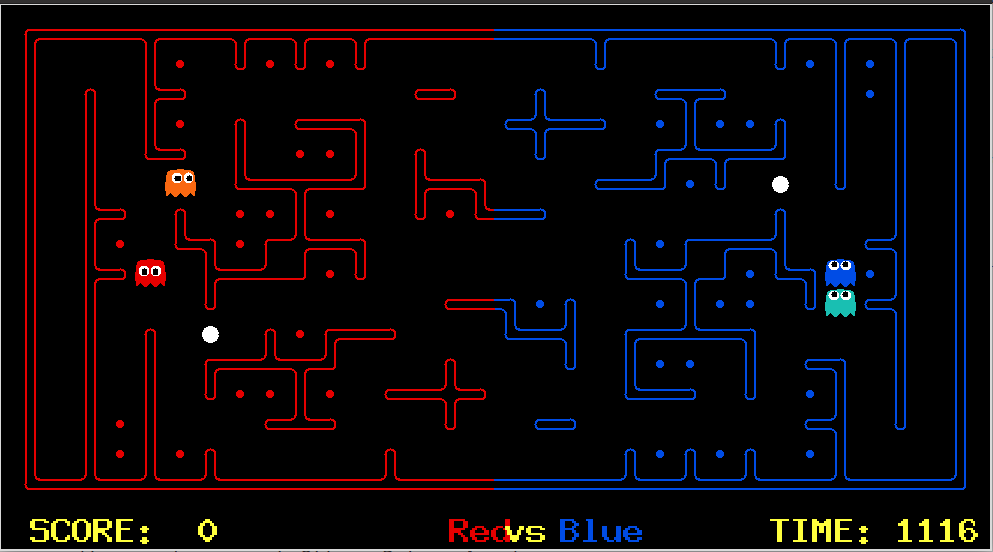
\includegraphics[width =.8\textwidth]{pacman.png} 
    \caption{Berkeley's Pac-Man environment in action.}
\end{figure}



The project code is developed in a modular way, so that users can work at different levels depending on their objective. There are three different modules:

\begin{description}
    \item [Agent development]: the source code of a participating agent is contained in a \texttt{github} repository. Each participating team will build a single repository. The \href{https://github.com/aig-upf/pacman-agent}{Pacman Agent} defines a basic template of an agent behavior.

    \item [Local tournament]:
    The (\href{https://github.com/aig-upf/pacman-contest}{Pacman Contest}) module contains the scripts needed to run a custom tournament locally, independently of the tournaments organized by UPF.

    \item [UPF tournament]:
    The \href{https://github.com/aig-upf/pacman-eutopia}{Pacman Eutopia} is the module used by tournament organizers at UPF. Participating organizations do not need to contribute to this module.
\end{description}

Currently, the framework supports a running mode based on \emph{events}. This means 
that tournaments are run at UPF according to prespecified dates between the tournament participants. A different mode with results continuously being updated is left for future versions of the framework.



\section{Rules of Pacman Capture the Flag}
\subsection{Layout}
The Pacman map is now divided into two halves: blue (right) and red (left). Red agents (which all have even indices) must defend the red food while trying to eat the blue food. When on the red side, a red agent is a ghost. When crossing into enemy territory, the agent becomes a Pacman.

\subsection{Scoring}
As a Pacman eats food dots, those food dots are stored up inside of that Pacman and removed from the board. When a Pacman returns to his side of the board, he ``deposits'' the food dots he is carrying, earning one point per food pellet delivered. Red team scores are positive, while Blue team scores are negative.

If Pacman is eaten by a ghost before reaching his own side of the board, he will explode into a cloud of food dots that will be deposited back onto the board.

\subsection{Eating Pacman}
When a Pacman is eaten by an opposing ghost, the Pacman returns to its starting position (as a ghost). No points are awarded for eating an opponent.

\subsection{Power Capsules}
If Pacman eats a power capsule, agents on the opposing team become ``scared'' for the next 40 moves, or until they are eaten and respawn, whichever comes sooner. Agents that are ``scared'' are susceptible while in the form of ghosts (i.e. while on their own team's side) to being eaten by Pacman. Specifically, if Pacman collides with a ``scared'' ghost, Pacman is unaffected and the ghost respawns at its starting position (no longer in the ``scared'' state).

\subsection{Observations}
Agents can only observe an opponent's configuration (position and direction) if they or their teammate is within 5 squares (Manhattan distance). In addition, an agent always gets a noisy distance reading for each agent on the board, which can be used to approximately locate unobserved opponents.

\subsection{Winning}
A game ends when one team returns all but two of the opponents' dots. Games are also limited to 1200 agent moves (300 moves per each of the four agents). If this move limit is reached, whichever team has returned the most food wins. If the score is zero (i.e., tied) this is recorded as a tie game.

\subsection{Computation Time}
We will run your submissions on the UPF cluster, SNOW.Tournaments will generate many processes that have to be executed without overloading the system. Therefore,  each agent has 1 second to return each action. Each move which does not return within one second will incur a warning. After three warnings, or any single move taking more than 3 seconds, the game is forfeit. There will be an initial start-up allowance of 15 seconds (use the \texttt{registerInitialState} function). If your agent times out or otherwise throws an exception, an error message will be present in the log files, which you can download from the results page.


\section{For students}
\label{sec:students}

Students need to first download the source code and install the required dependencies.\footnote{Commands expected to be used in an \textsc{Ubuntu} operative system and tested for version \textsc{Ubuntu 22.04}.}

\subsection{Setting up the agent and contest frameworks}

Step by step:
\begin{enumerate}
    \item Clone the repository to download all the necessary code.\\
    \texttt{git clone git@github.com:aig-upf/pacman-agent.git}
    \item Move to the created directory.\\
    \texttt{cd pacman-agent/}
    \item Create a virtual environment.\\
    \texttt{python3.8 -m venv venv}
    \item Activate the virtual enviroment.\\
    \texttt{source venv/bin/activate}
    \item Pull the contest framework.\\
    \texttt{git submodule update --init --remote}
    \item Install the contest framework and required python libraries.\\
    \texttt{cd pacman-contest/}\\
    \texttt{pip install -e .} \\
    \texttt{pip install -r requirements.txt} 
    \item Finally, move to the directory containing the main file (\texttt{capture.py}) to run a match.\\
    \texttt{cd src/contest/}
\end{enumerate}

\subsection{Getting Started}
By default, you can run a game with the simple \texttt{baseline\_team} that the staff has provided:
\\

\texttt{python capture.py}
\\

A wealth of options are available to you:
\\

\texttt{python capture.py --help}
\\

The code provides one sample team called \texttt{baseline\_team}, contained in a python script named \texttt{baseline\_team.py} in \texttt{src/contest} folder. It is chosen by default as both the red and blue team, but as an example of how to choose teams:
\\

\texttt{python capture.py -r baseline\_team -b baseline\_team}
\\

which specifies that the red team \texttt{-r} and the blue team \texttt{-b} are both created from \texttt{baseline\_team.py}. \\

Once this last step is working, we can start running games between our custom agents, or between a custom agent and the \texttt{baseline\_team}. To do this, we will save our agent's directory in the \texttt{src/contest/agents/} folder. Inside this folder we will have our directory, which can have any name. As an example, let's imagine that we have two agents, \texttt{team\_name\_1} and \texttt{team\_name\_2}. Each of these folders contains an agent, in a script called \texttt{my\_team.py}.
An executable example is provided in the framework: 
\\

\texttt{python capture.py -r agents/team\_name\_1/my\_team.py -b agents/team\_name\_2/my\_team.py}
\\

We could also compare our agent against the \texttt{baseline\_team}, by running
\\

\texttt{python capture.py -r agents/team\_name\_1/my\_team.py -b baseline\_team}
\\

There is also an option to record the game and some log info by adding the flags \texttt{--record} and \texttt{--record-log} to the previous command. 

\texttt{python capture.py -r agents/team\_name\_1/my\_team.py -b baseline\_team --record --record-log}
\\

The previous command will save the data in the following files:
\begin{itemize}
    \item Log: \texttt{www/contest\_default/logs/match\_0.log}
    \item Replay: \texttt{www/contest\_default/replays/match\_0.replay}
    \item Score: \texttt{www/contest\_default/scores/match\_0.json}
\end{itemize}

Finally, a match can be replayed from a \texttt{*.replay} file. Using the one generated in the previous execution, we can run it as follows:

\texttt{python capture.py --replay=www/contest\_default/replays/match\_0.replay}

\subsection{Building your agent}
In the root folder do the following:

\begin{enumerate}
    \item Create in \texttt{my\_team.py} a class with the name of your agent that inherits from \texttt{CaptureAgent}, e.g. class \texttt{ReflexCaptureAgent(CaptureAgent):}
    \item In the new class, override the \texttt{def choose\_action(self, game\_state):} function to return the best next action (check the given source code example).
    \item (Optional) Add any other functions to the class for reasoning / learning and improving your agents decision which could also use other code sources in the same folder.
\end{enumerate}

If you want to debug your agent, provide the local route to \texttt{capture.py}, e.g., \texttt{python capture.py -r baseline\_team -b ../../../my\_team.py} for your agent to play against the \texttt{baseline\_team}.

\newpage

\end{document}
